\section{UML Diagrams}
\subsection{Framework implementation}
The \vs is based on stack representation, in particoular is composed by a vehicles which a transceiver for send and receive messages on the network and under that leve a security box which use the security implementation which you have set during simulation.
\subsection{Class Diagram}
\begin{figure}[ht]
% If the picture uses fonts of the correct size (10 ... 12 pt)
% then can be included without scaling
%\centerline{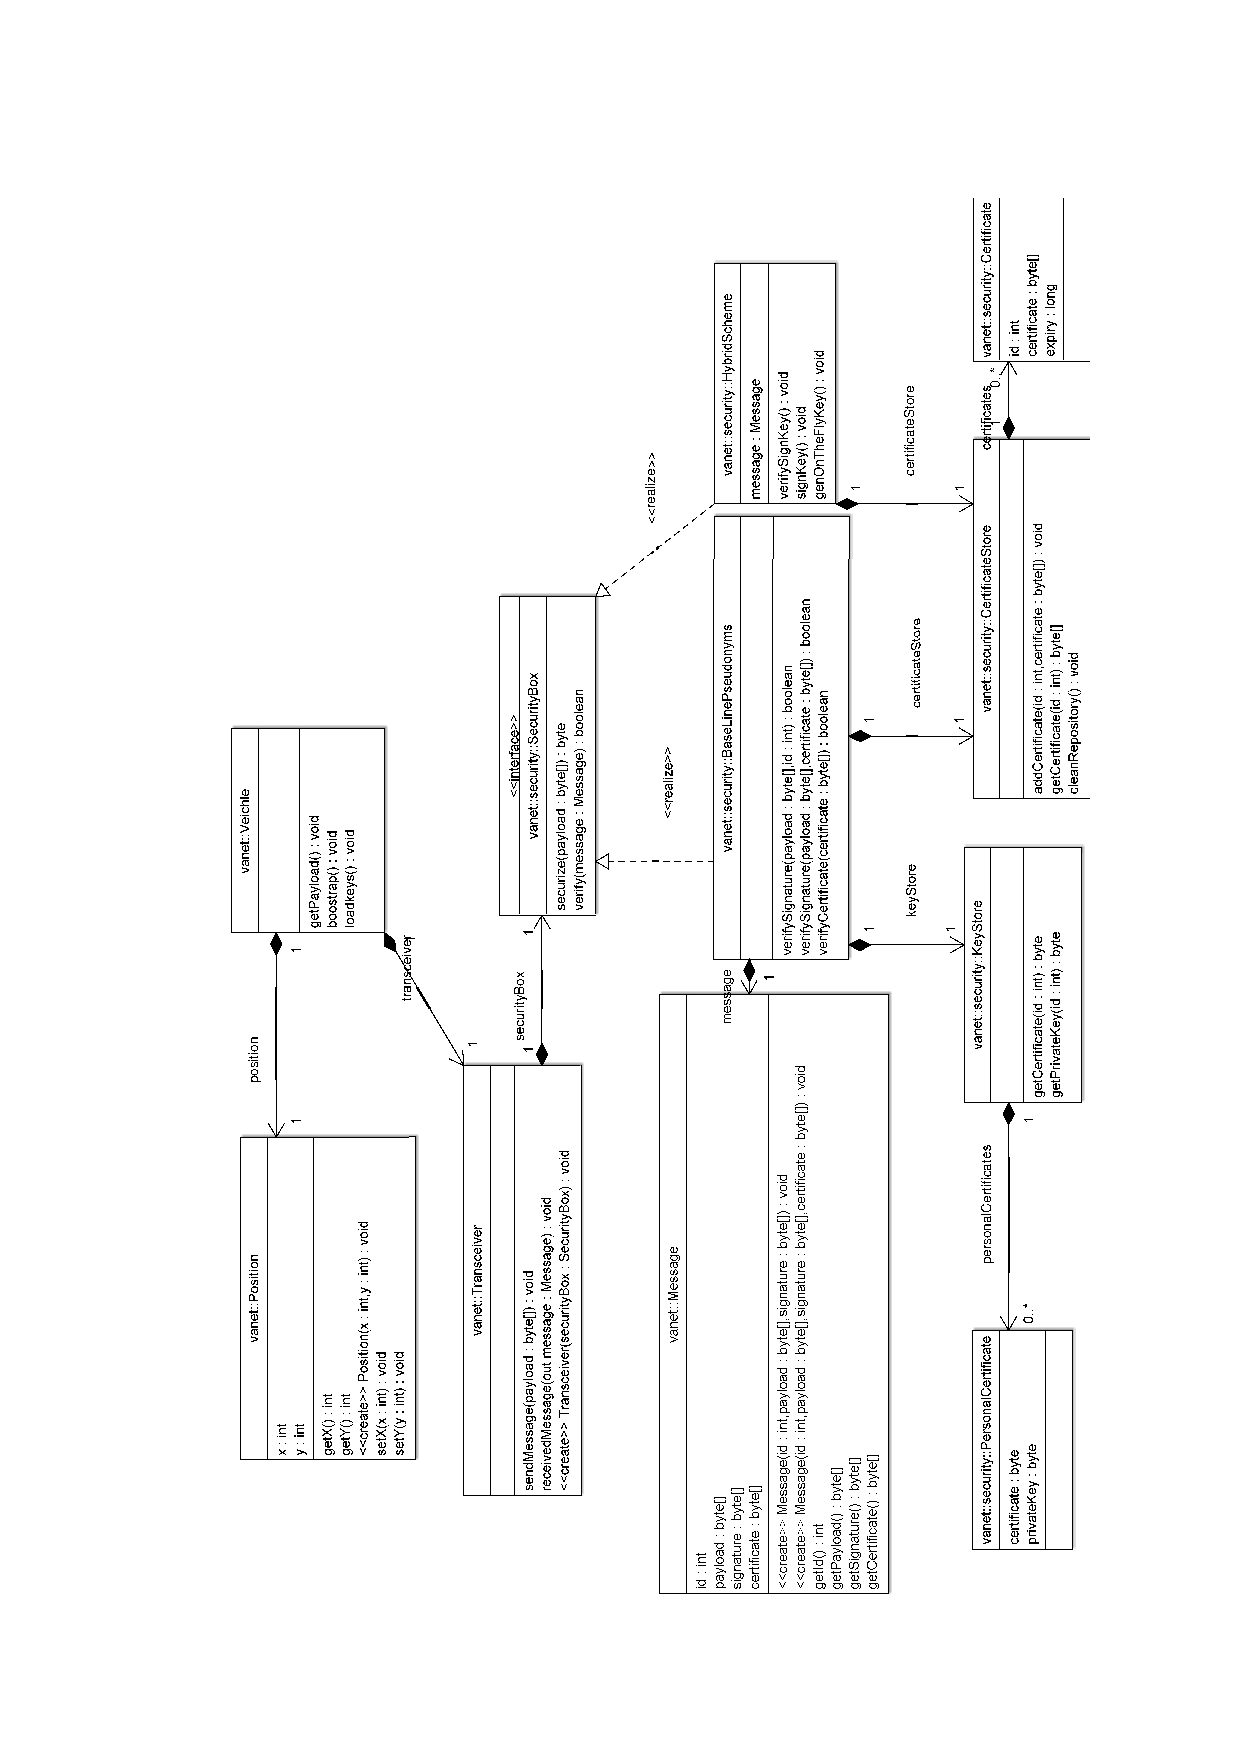
\includegraphics{class_diagram.pdf}}
% otherwise see the example in the following (commented out) line
% to scale it relatively to the page width
\centerline{\includegraphics[width=0.9\textwidth]{vanet_class.pdf}}
\caption{Class Diagram}
\label{fig:class_diagram}
\end{figure}
\begin{figure}[ht]
% If the picture uses fonts of the correct size (10 ... 12 pt)
% then can be included without scaling
%\centerline{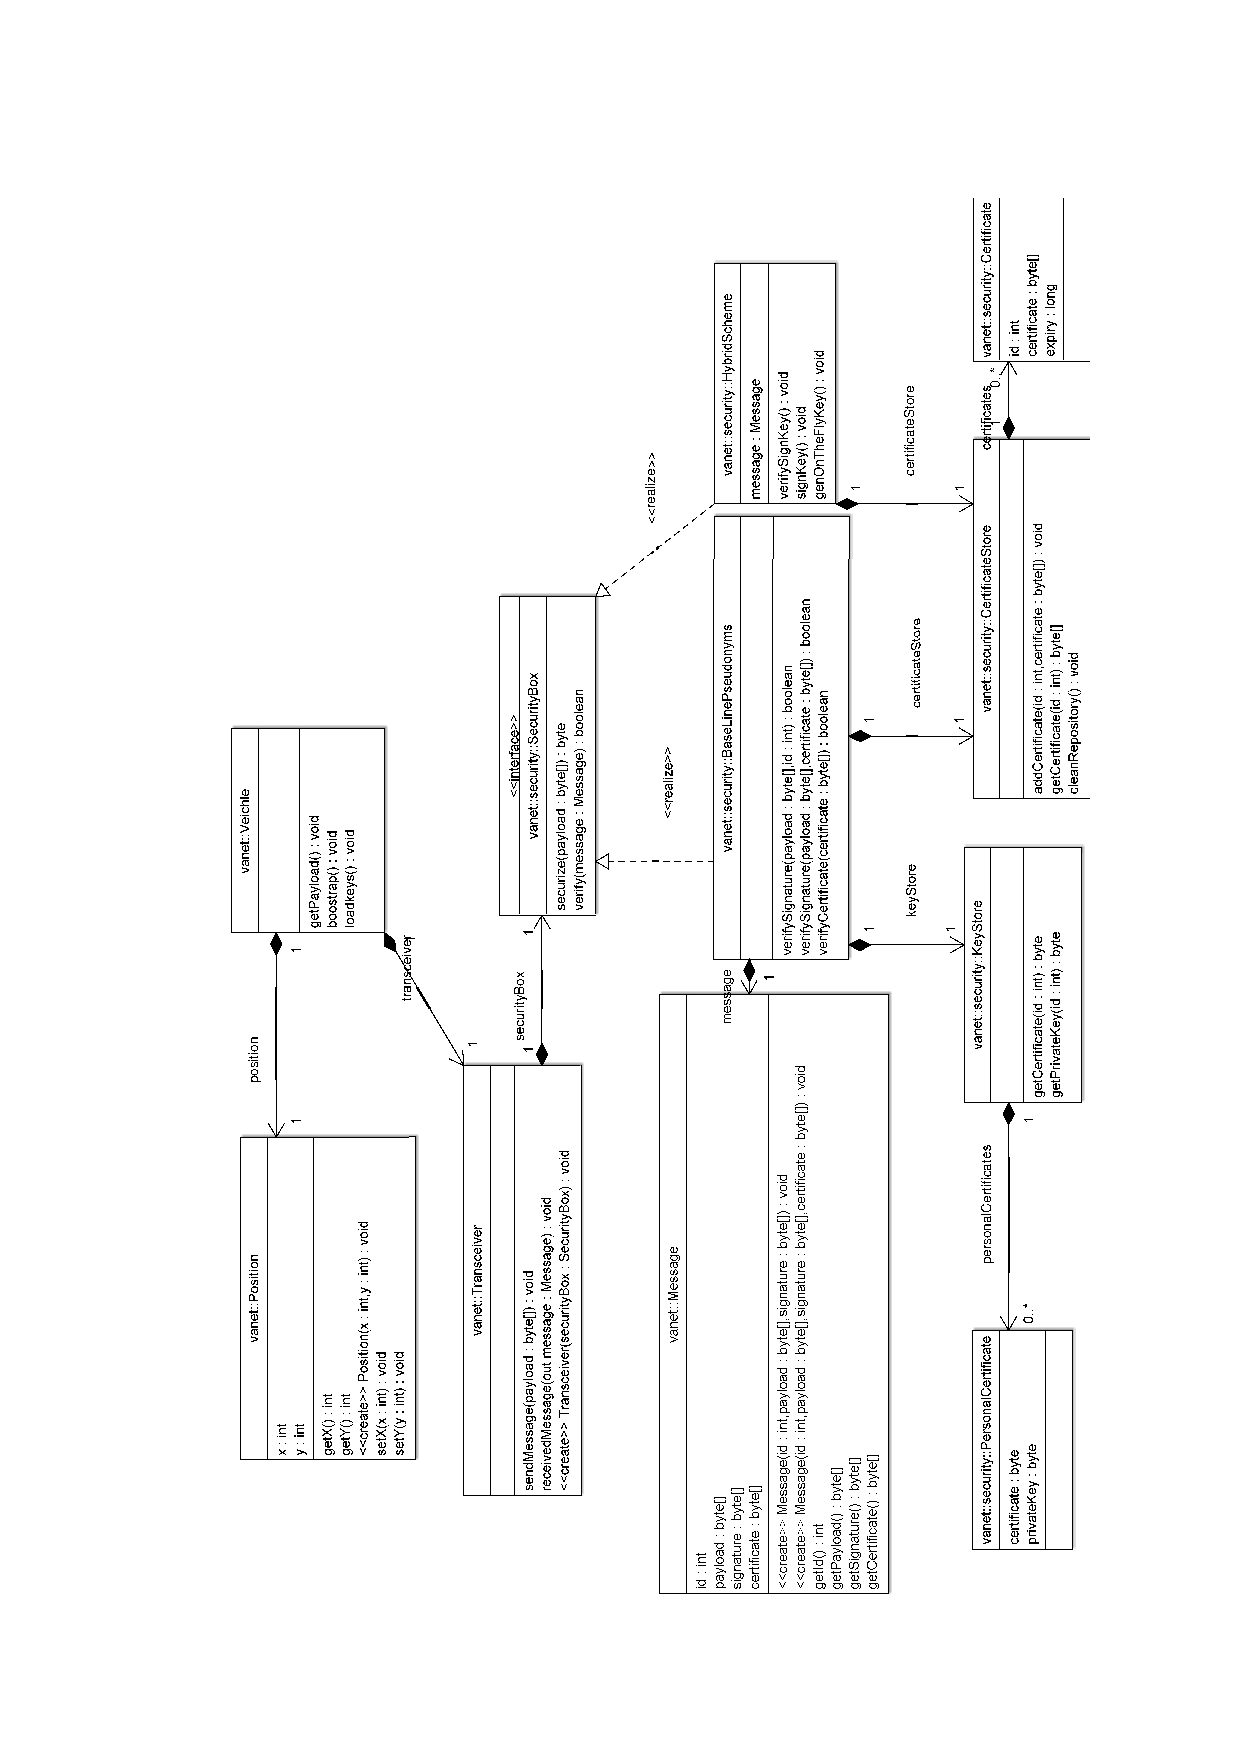
\includegraphics{class_diagram.pdf}}
% otherwise see the example in the following (commented out) line
% to scale it relatively to the page width
\centerline{\includegraphics[width=0.9\textwidth]{baseline_send_message.pdf}}
\caption{Sequence Diagram \baseline securize and send message}
\label{fig:sequence_send_baseline}
\end{figure}
\subsection{Sequence Diagrams}
\begin{figure}[ht]
% If the picture uses fonts of the correct size (10 ... 12 pt)
% then can be included without scaling
%\centerline{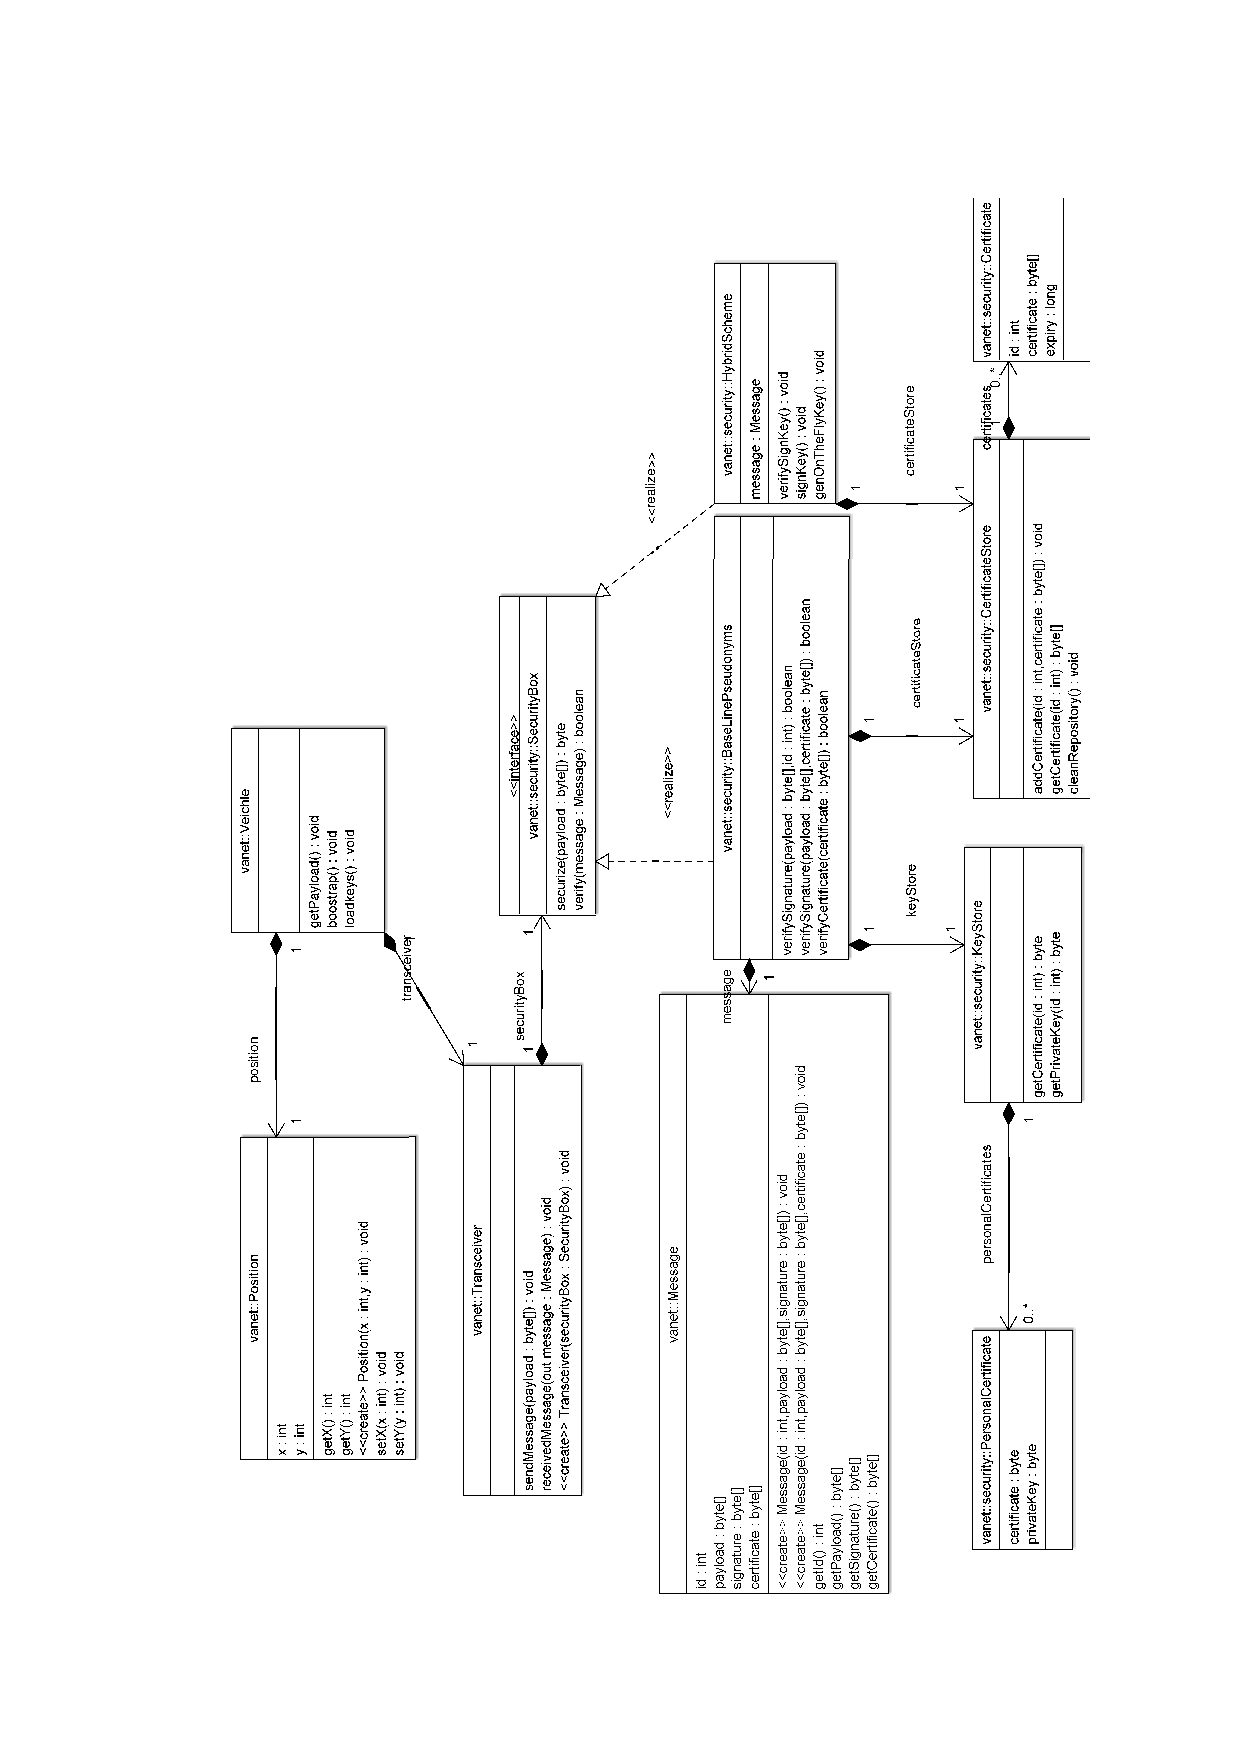
\includegraphics{class_diagram.pdf}}
% otherwise see the example in the following (commented out) line
% to scale it relatively to the page width
\centerline{\includegraphics[width=0.9\textwidth]{baseline_receive_message.pdf}}
\caption{Sequence Diagram \baseline receive and check message}
\label{fig:sequence_receive_baseline}
\end{figure}
\begin{figure}[ht]
% If the picture uses fonts of the correct size (10 ... 12 pt)
% then can be included without scaling
%\centerline{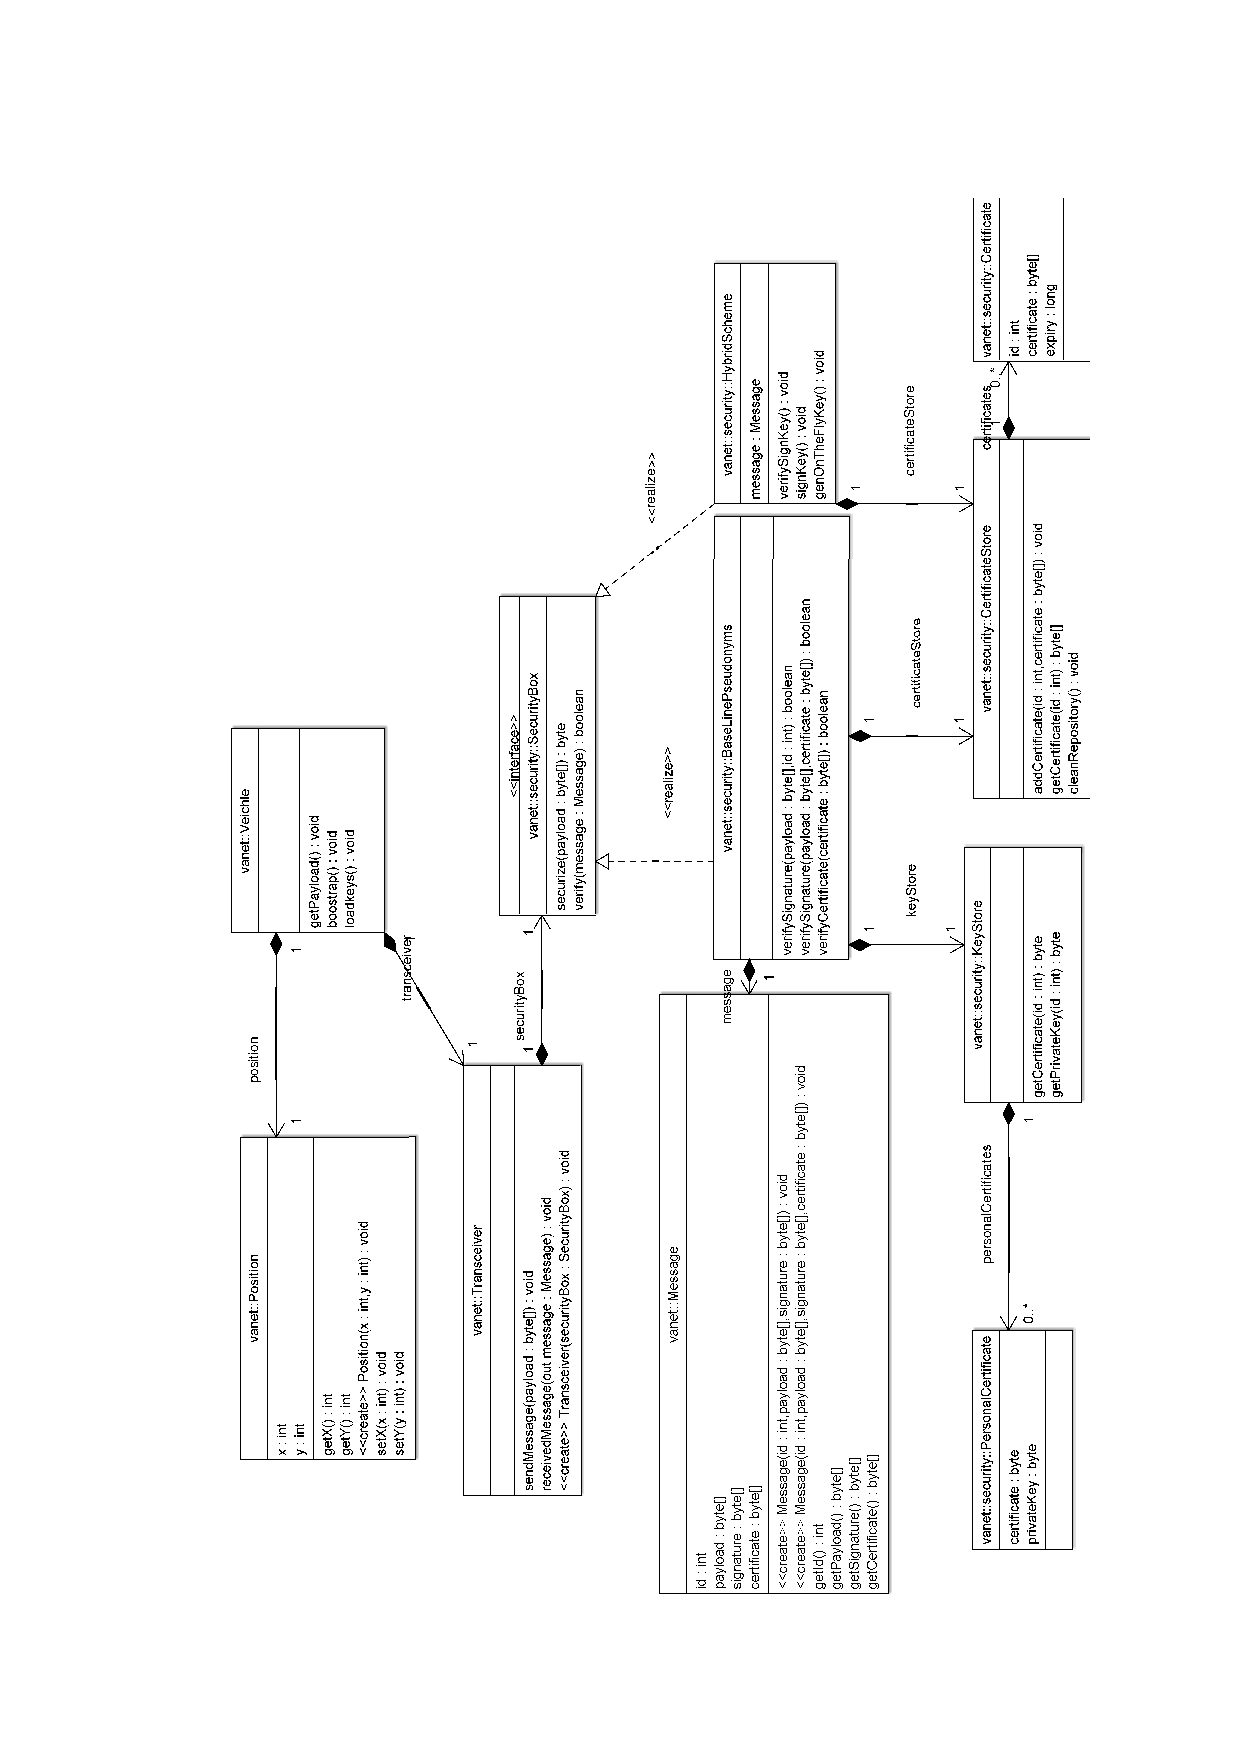
\includegraphics{class_diagram.pdf}}
% otherwise see the example in the following (commented out) line
% to scale it relatively to the page width
\centerline{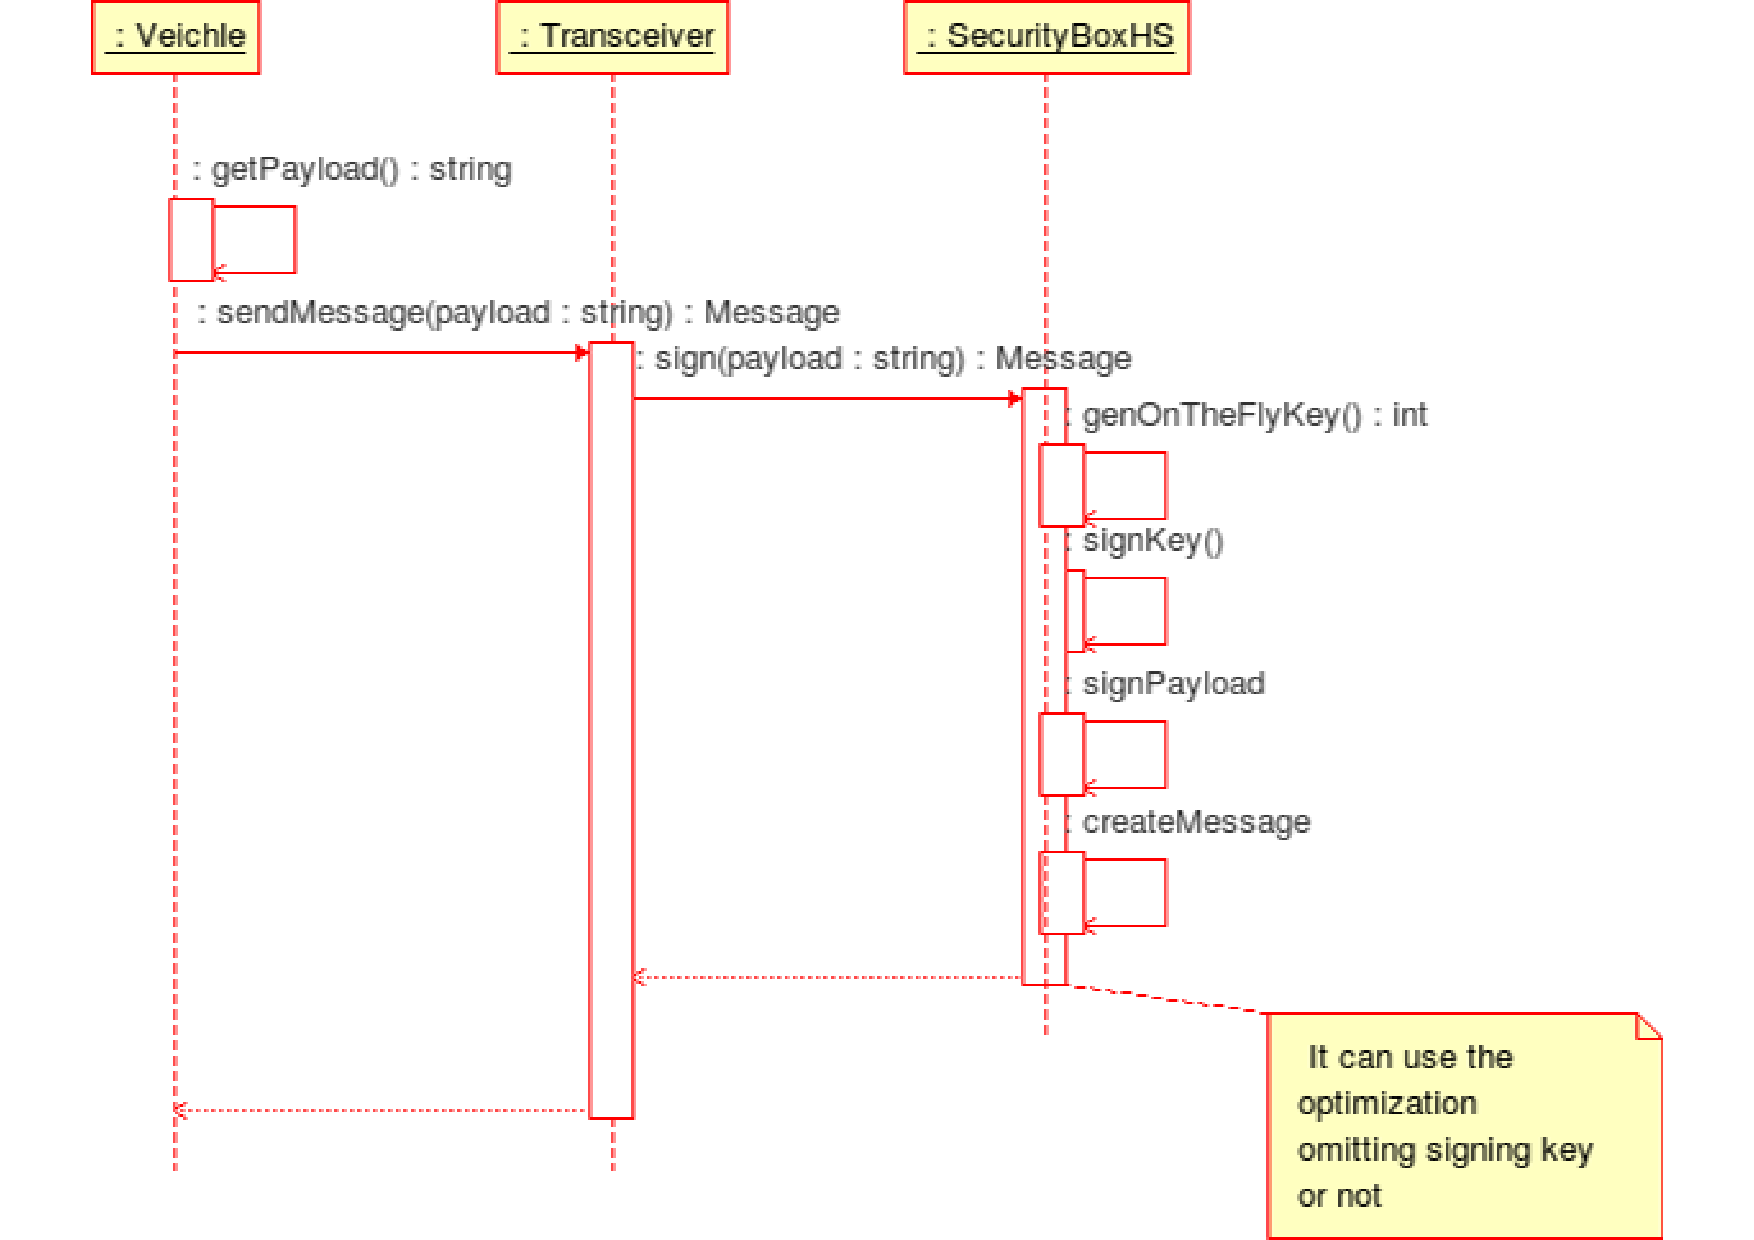
\includegraphics[width=0.9\textwidth]{hybrid_scheme_send_message.pdf}}
\caption{Sequence Diagram \hybrid securize and send}
\label{fig:sequence_send_hybridscheme}
\end{figure}
\begin{figure}[ht]
% If the picture uses fonts of the correct size (10 ... 12 pt)
% then can be included without scaling
%\centerline{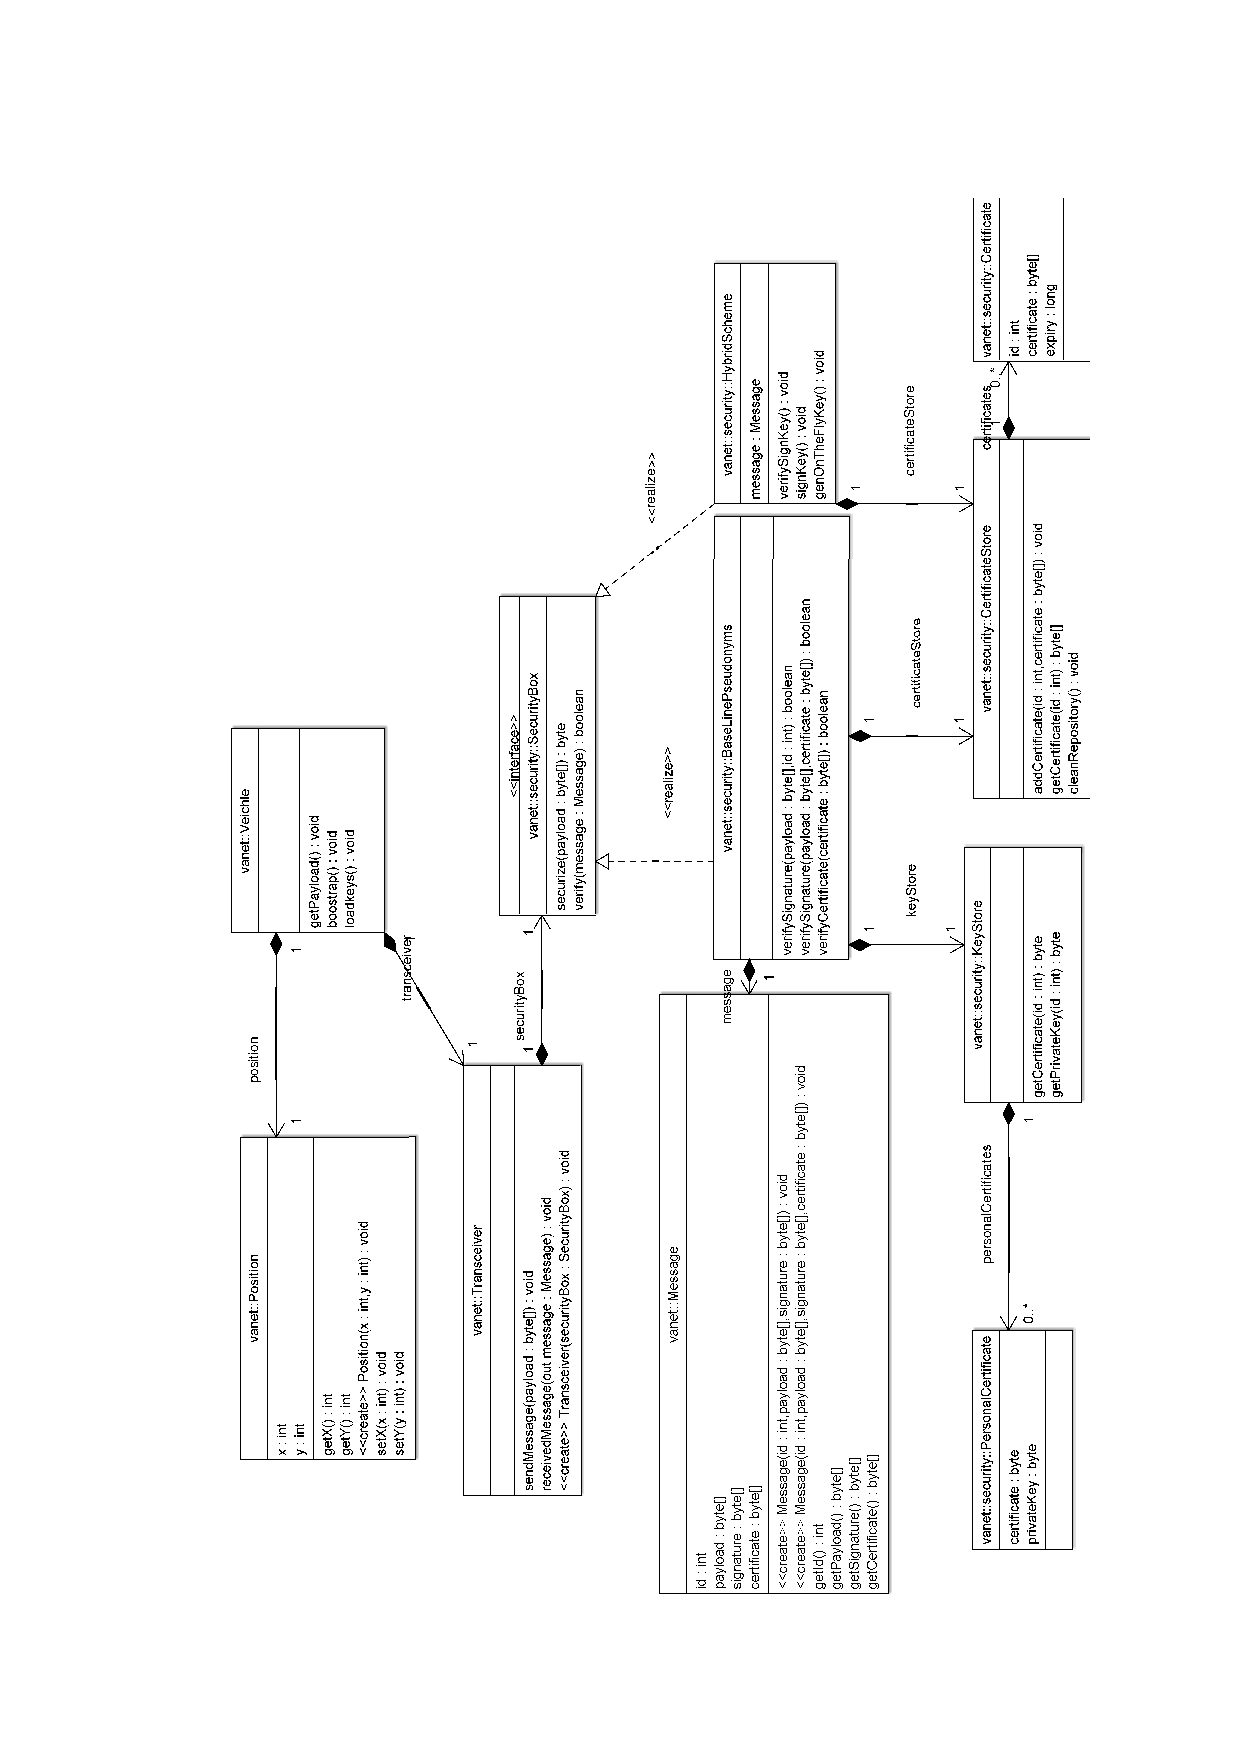
\includegraphics{class_diagram.pdf}}
% otherwise see the example in the following (commented out) line
% to scale it relatively to the page width
\centerline{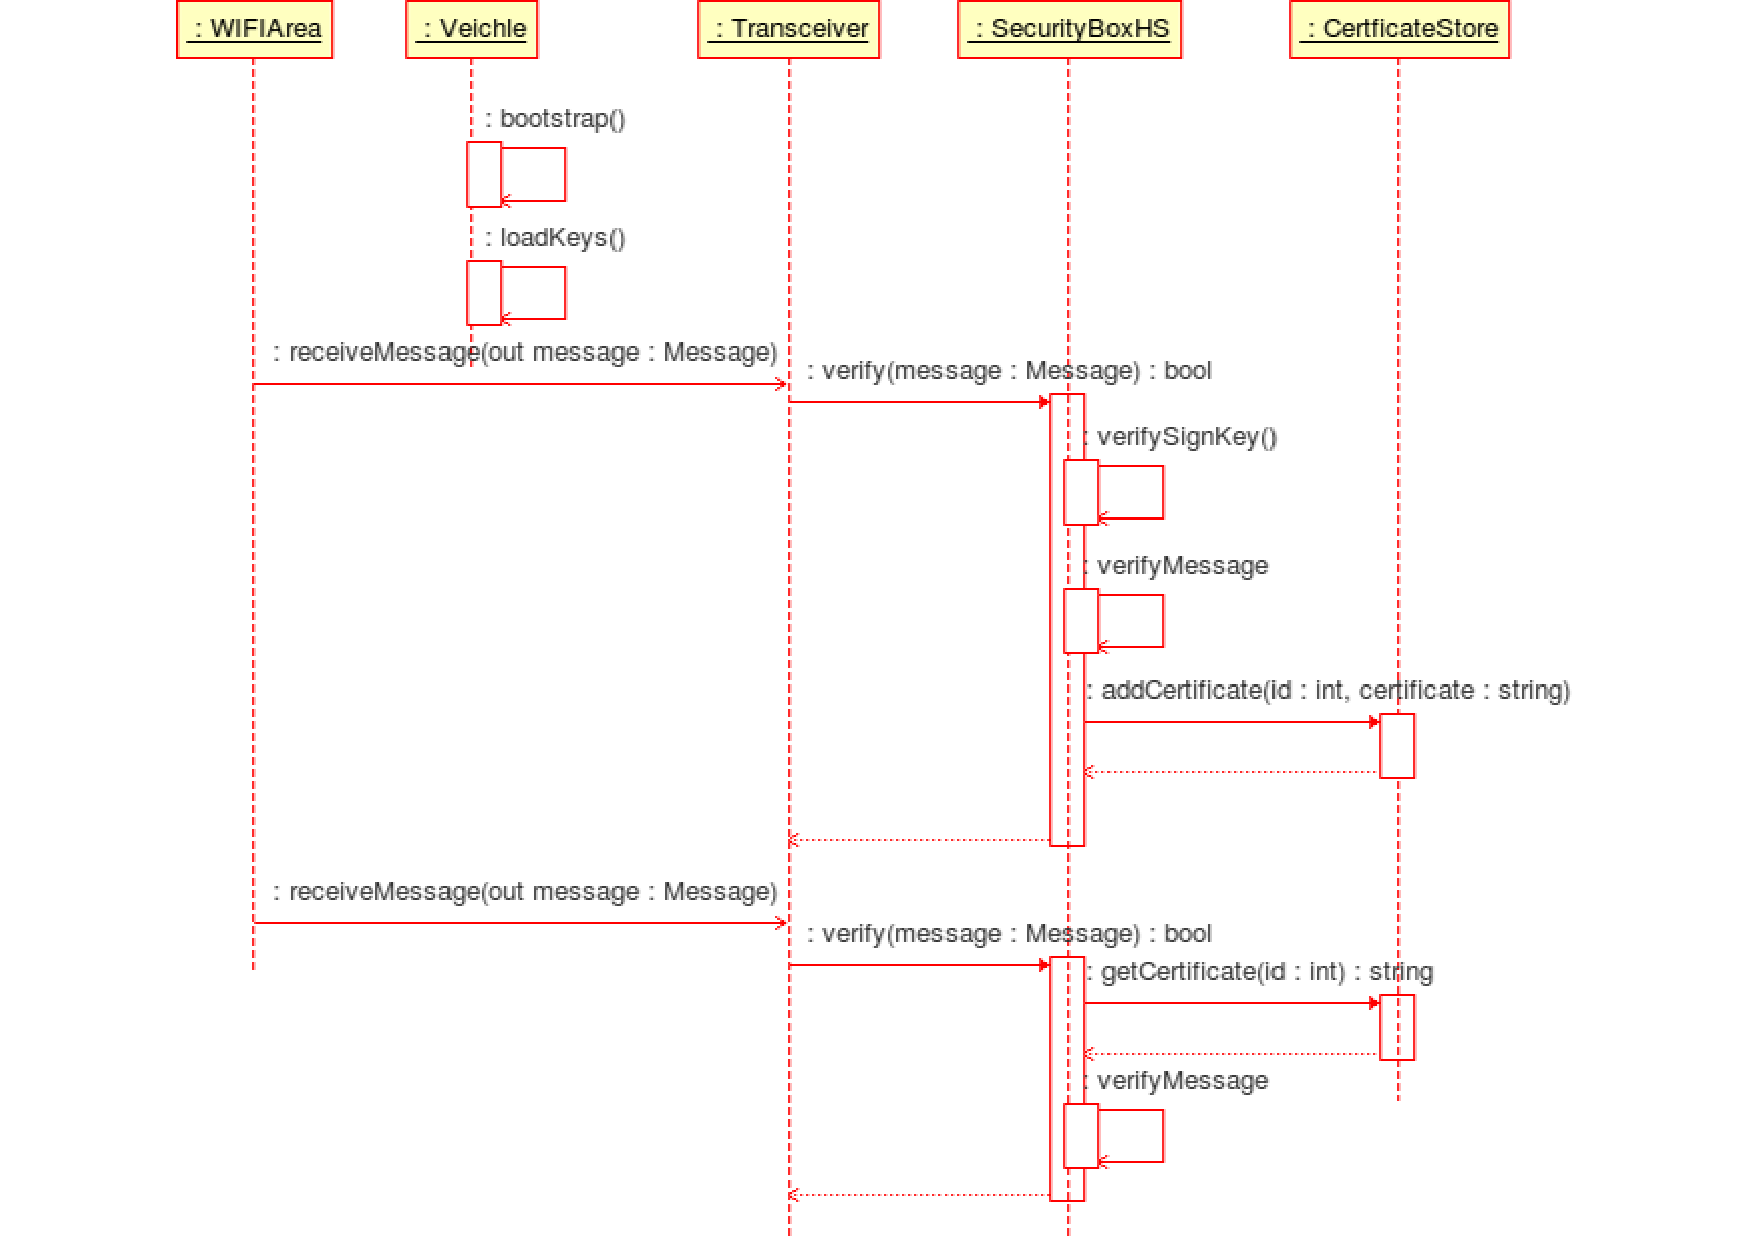
\includegraphics[width=0.9\textwidth]{hybrid_scheme_receive_message.pdf}}
\caption{Sequence Diagram \hybrid receive and check}
\label{fig:sequence_receive_hybridscheme}
\end{figure}